\documentclass[12pt,a4paper]{book}
\usepackage[minitoc]{teach}
\usepackage[utf8]{inputenc}
\usepackage[french]{babel}
\usepackage[T1]{fontenc}
\usepackage{amsmath}
\usepackage{amsfonts}
\usepackage{amssymb}
\usepackage{graphicx}
\renewcommand{\headrulewidth}{0pt}
\renewcommand{\footrulewidth}{0pt}
\fancyfoot[C]{\thepage}


\author{YAWO Kossi Atsu}
\newcommand{\prof}{YAWO Kossi Atsu}
\newcommand{\matiere}{PHYSIQUE- CHIMIE}
\newcommand{\classe}{6$^{ème}$}
\title{Mes devoirs de Mathématiques}
\begin{document}
\begin{td}{\matiere}{\classe}{24 mai 2019}{\prof}
\end{td}

\begin{td}{\matiere}{\classe}{24 mai 2019}{\prof}

\end{td}

\begin{td}{\matiere}{\classe}{24 mai 2019}{\prof}

\end{td}

\begin{td}{\matiere}{\classe}{24 mai 2019}{\prof}

\end{td}

\newpage
\begin{devoir}{COMPOSITION DU TROISIÈME TRIMESTRE}{\matiere}{\classe}{1}{1H 30}{29 mai 2019}{\prof}
\begin{exo}[4,5]
\begin{enumerate}
\item Schématise un circuit électrique comportant un générateur, une lampe, un interrupteur ouvert et un moteur.
\competence{schématiser un circuit électrique}{1.5}
\item Le moteur fonctionne- t- il? pourquoi?
\competence{connaître le rôle du courant électrique et celui d'un interrupteur}{1}
\item On ferme l'interrupteur. Quels évènements note- t- on?
\competence{connaître le fonctionnement d'une lampe et d'un moteur}{2}
\end{enumerate}

\vspace{0.2cm}
\end{exo}

\begin{exo}[4]
Ariane a pesé un objet et a trouvé $450g$.
\begin{enumerate}
\item Que représente $450g$ pour cet objet?
\competence{reconnaître une masse à l'aide de l'unité}{1}
\item Définir cette grandeur.
\competence{définir la masse}{1}
\item Quel instrument de mesure a- t- elle utilisé?
\competence{connaître l'instrument de mesure de la masse}{1}
\item Quelles sont les masses marquées possibles qu'elle aurait utilisées?
\competence{manipuler les masses marquées}{1}
\end{enumerate}

\vspace{0.2cm}
\end{exo}

\begin{exo}[7]
On brûle le soufre dans $1l$ d'air.
\begin{enumerate}
\item Donne le nom du produit obtenu.
\item Comment peut- on reconnaître ce gaz?
\competence{nommer et identifier le produit formé au cours de la combustion du soufre}{2}
\item Calcule le volume d'oxygène contenu dans le flacon.
\competence{utiliser la composition en volume de l'air}{1}
\item La masse du soufre augmente ou diminue- t- elle dans le flacon? Pourquoi?
\competence{lois d'un réaction chimique}{1}
\item Écris la formule chimique de cette réaction.
\competence{écrire la formule chimique de la combustion du soufre}{1}
\item Avant la combustion la masse du soufre est de $32,6g$. Après le combustion, sa masse est $32,2g$. Calcule la masse du soufre disparue.
\competence{calcule la masse consommée d'un réactif}{1}
\item Calcule la masse du soufre qui peut brûler dans $1l$ d'air.
\competence{utiliser la proportionnalité pour calculer une masse}{1}
\end{enumerate}

\vspace{0.2cm}
\end{exo}

\begin{exo}[4,5]
Sur la figure ci-dessous, les piles sont identiques et ont chacune $1,5V$. Sur le culot de lampe, on peut lire $7,2V$.\\
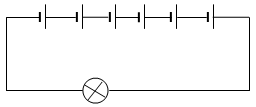
\includegraphics[scale=0.9]{images/compo3_2019_img1.png}
\begin{enumerate}
\item Que représente la valeur $1,5V$ inscrite sur une pile?
\competence{identifier la tension d'une pile}{0.5}
\item Que représente la valeur $7,2V$ inscrite sur une lampe?
\competence{identifier la tension d'usage d'une lampe}{0.5}
\item \begin{enumerate}
\item S'agit-il d'une bonne association? Pourquoi?
\item Quelle nom donne- t- on à cet type d'association?
\competence{reconnaître une association en concordance}{1.5}
\item Sous quelle tension la lampe est- elle alimentée? Comment brille- t- elle?
\competence{calculer la tension d'une association de pile}{0.5}
\end{enumerate}
\item Reproduis le schéma en associant les piles en concordance. Quelle sera alors la nouvelle tension? Comment brillerait la lampe?
\competence{réaliser le schéma d'une association de pile en concordance et calculer la tension}{1.5}
\end{enumerate}

\vspace{0.2cm}
\end{exo}

\tableofcompetences
\end{devoir}

\end{document}
